\documentclass[../Text/00main.tex]{subfiles}
\graphicspath{{../}}

\begin{document}


Earthquakes pose a destructive natural hazard with a large socio-economic impact, and their timing or consequences remain hard to predict. Seismic hazard assessment is an important factor for infrastructural planning and disaster management in seismically active and densely populated regions. Studying the potential effects of an event can make the disaster response more effective and populated areas more resilient. Various methods can be used to assess the impact of a potential future earthquake. For many years, empirical Ground Motion Prediction Equations (GMPEs) were developed on basis of historical seismic data, and were extrapolated to regions in the world with less coverage or knowledge of the subsurface. In the recent years, the coverage and resolution of subsurface models, through full waveform inversion has grown substantially, i.e. the Collaborative Seismic Earth Model (CSEM) \citep{afanasiev2016foundations}. In combination with the growing computational resources of large high-performance computing centres (HPCs), this allows for numerical simulation of large seismic events in regional domains. Numerical modelling of earthquakes forms a powerful tool with the potential to produce estimates for seismic hazard assessment, and if accurate enough, can help mitigate damage or allow for adequate response by the authorities.  

The frequency content of an earthquake that is relevant for most civil structures stretches 1-10 Hz \cite{chandler1997dynamics}. As availability of high-resolution Earth models and computational power increases, routine simulations of potential events, or rapid post-event simulations, become less computationally prohibitive. Various efforts are being taken to push the frequency limit of deterministic seismic simulations up to higher frequencies, recently up to 8 Hz e.g. \cite{rodgers_broadband_2019}, \cite{he2015simulation}. This is also made possible by the increasing number of subsurface models obtained by full-waveform inversion. 

\subsection{ChEESE}

This project is written in the context of urgent seismic simulations, which is part of Pilot 1 of the Center of Excellence (CoE) in the Solid Earth (ChEESE). The ChEESE project develops flagship codes for the future Exascale and pre-Exascale high-performance computing centres (HPCs). The aim of urgent seismic simulations is to promptly start a workflow of simulations to characterise a large seismic event after it has occurred. This would require urgent access to HPCs and could deliver ground motion estimates of affected areas, and has a potential to aid regional disaster management.  The first step of this urgent simulation workflow entails the characterisation of the seismic source as a point source: the centroid moment tensor (CMT). However, this point-source approximation is not accurate for the large events that the project aims to simulate. Following the successful determination of the point-source mechanism, more realistic kinematic rupture simulations such as \cite{graves_kinematic_2016} can be set to work. These more complex simulation call for more parameters, entailing more uncertainty. This prompts us to first dive into the effects of uncertainty on the CMT solution. 

\subsection{Research goals}

The spatial distribution of ground motion can be studied for adequate seismic hazard assessment and disaster response. Proxies or intensity measures (IM) describing the peak amplitudes of an event, such as the Peak Ground Acceleration (PGA) and Peak Ground Velocity (PGV) are often evaluated in seismic risk analysis and earthquake engineering. Other proxies quantify the spectral content and the duration of the earthquake. Uncertainties in simulation of earthquakes, due to simplifications of reality or uncertainties of input parameters, can affect the spatial variability of these intensity measures. Major contributors to modelling uncertainty are the source model, resolution of the subsurface model, and related to this, contribution of relatively small-scale basin structures to site- and path-effects, e.g. \cite{}. Additionally, the inclusion of realistic domain components such as topography, bathymetry and modelling of large water bodies \cite{afanasiev2019effect}. Uncertainty in these modelling parameters can cause variability in the ground motion patterns, and this may have great impact on the spatial determination of seismic hazards. This study focuses on how the spatial variability of ground motion proxies is affected by uncertainty in the source model and inclusion of model domain complexities, such as topography and ocean. 

Catalogues such as the Global Centroid Moment Tensor (GCMT, \cite{ekstromdziewo}) catalogue provide information about the earthquake mechanism and represent the source as a Centroid Moment Tensor (CMT). The catalogue provides the strike, dip and rake of the nodal planes and the six individual moment tensor components, as well as their uncertainties.  Especially with the rapid source inversions done in the urgent seismic simulation context, location, depth and composition of the source are subject to uncertainty. The subsurface model and source estimate are important factors for the performance of a numerical earthquake simulation. We employ a high-resolution subsurface model of Western Turkey (seev\cite{cubuk-sabuncu_3-d_2017}), obtained by full waveform inversion and produced in the context of the community seismic earth models. A case study is conducted on the North Anatolian Fault in the sea of Marmara, just south of Istanbul. This is a densely populated region, with more than 13 million inhabitants. It lies in one of the most active seismic regions on the continental rims of the Anatolian and Eurasian plates and is facing perhaps one of the highest seismic hazards on Earth.


\section{Study region} \label{CH1sec:Tectonics}

\subsection{Tectonics}
 \begin{figure}
     \centering
     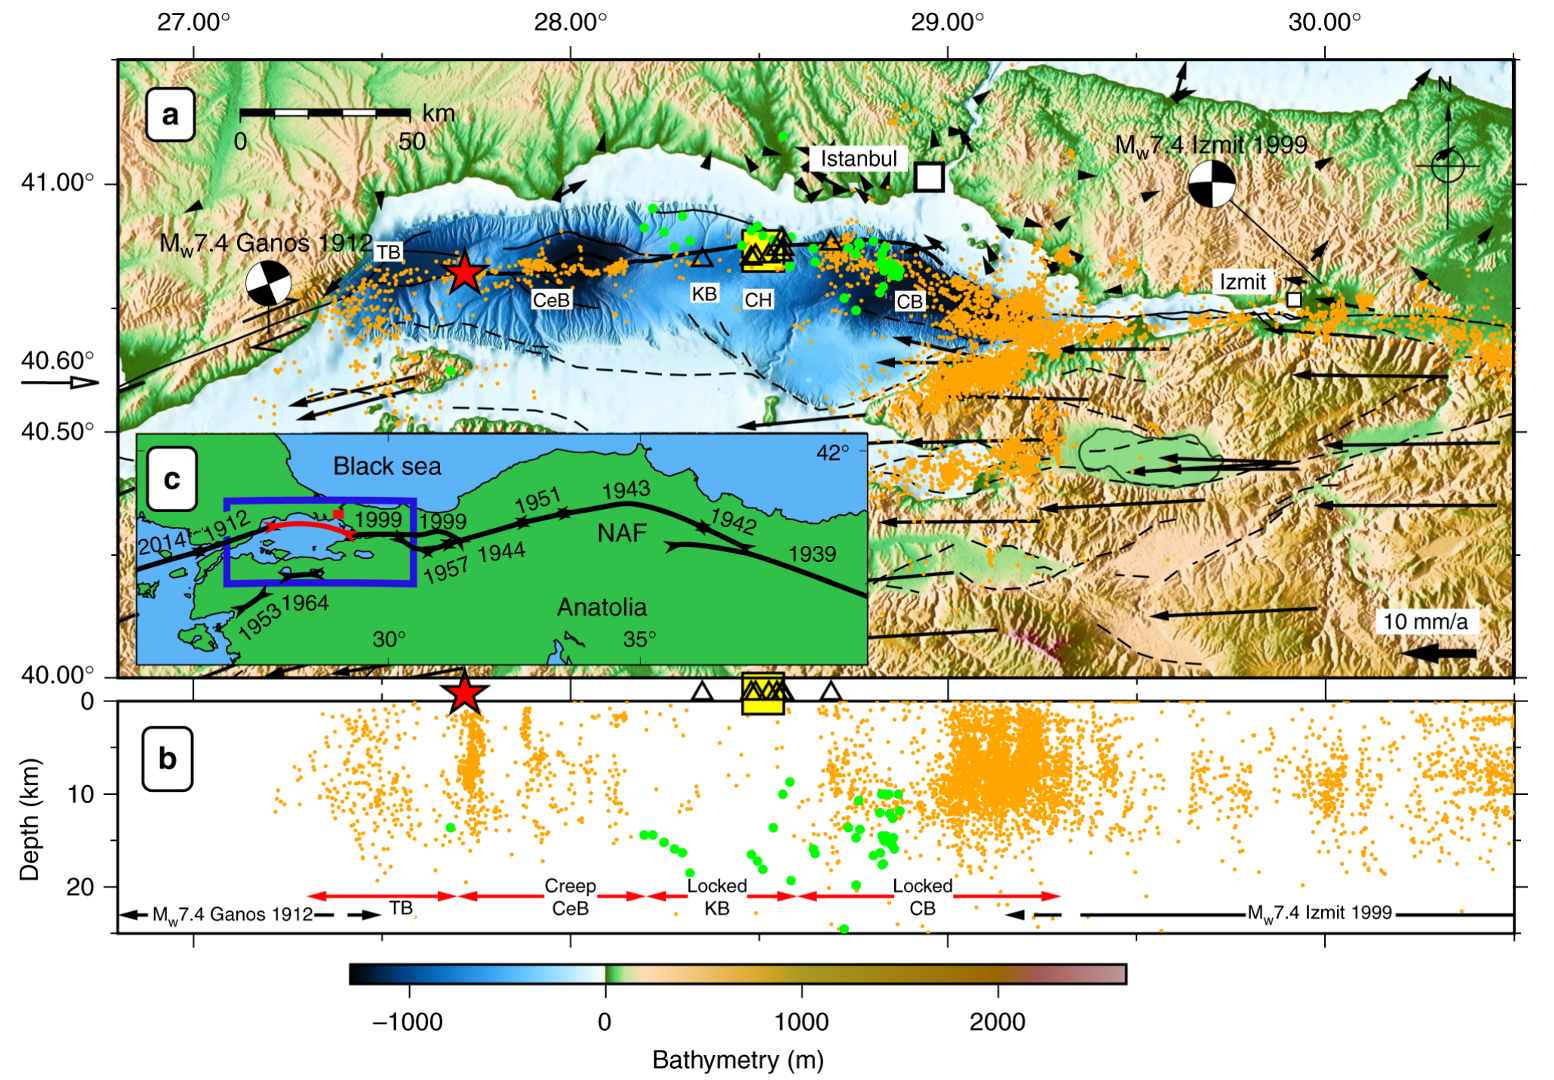
\includegraphics[width=.5\linewidth]{images_methods/bonhoff_integrative.png}
     \caption{\cite{bohnhoff_maximum_2016}}
     \label{fig:bonhoffintegrative}
 \end{figure}


Western Turkey constitutes a tectonically active study area. The tectonics are a result of the northward-moving African plate, subducting under the Eurasian plate in the Aegean region, and the Arabian plate to the south-east pushing westward. The Anatolian plate is locked between the three large continental plates, and is being pushed Westwards, whilst rotating in a counter-clockwise fashion \cite{rotstein1984counterclockwise}. The main intra-plate friction caused by this movement is created along the East- and North-Anatolian Fault zones. Figure (?) shows a sketch of the tectonic regime in the region, with the North-Anatolian Fault Zone (NAFZ) coming forward as the important feature. The seismic hazard map in Figure \ref{fig:hazmap} underlines this importance with a very high seismic risk. The NAFZ is a schoolbook example of a dextral strike-slip fault zone. It has a rich earthquake history, with the largest recent event being the $M_w 7.9$ Izmit and Dücze earthquakes in 1999. It has become clear that earthquakes occur sequentially, rupturing in segments along the fault-zone from east to west in the previous centuries \cite{bohnhoff_earthquake_2013},\cite{bulut_magnitudes_2019}. 

\subsection{Seismic hazard}

Since the 1999 Izmit and Dücze earthquakes, several medium-magnitude events have occurred along the Marmara segment of the NAFZ. However, a major ($> M_w 7.0$) rupture in this section of the fault zone has not occurred since 1766. The recent history of ruptures along the fault-zone reveals that as successive earthquakes move east to west along the NAFZ and have reached Izmit in 1999 as most recent western boundary, no successive major event in the Marmara sea region has occurred. This region, stretching along 150 km of the northern branch of the fault zone, has exhibited increased activity since 1999 \cite{bohnhoff_earthquake_2013}, and is believed to be capable of producing a $> M_w 7.0$ event in the near future. Consequently, stress buildup of this part fault-zone is being closely monitored. A distinct area of 30 km just south of Istanbul named the "Princess Island Segment", shows close to zero seismicity in the recent history (\cite{bohnhoff_earthquake_2013}) and has gained attention as the potential next rupture location in the recent years. The two hypotheses for the stress accommodation in this part of the fault zone are either slow seismic creep, or a completely locked regime with a large stress buildup. Monitoring of this segment is complicated by its submerged location. Recent efforts of characterising the regime in this region using ocean-bottom sensors, such as \cite{lange2019interseismic}, point increasingly towards a completely locked regime.

\begin{figure}
    \centering
    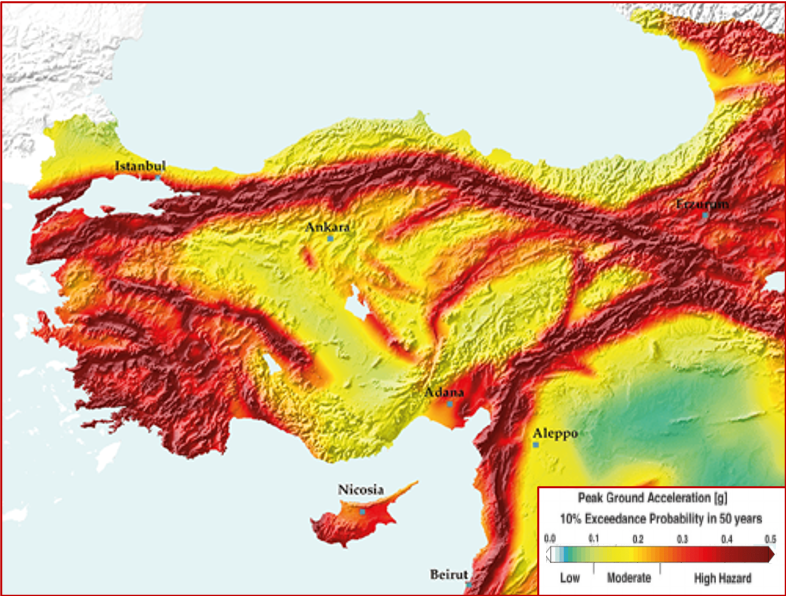
\includegraphics[width=0.5\linewidth]{images_methods/Hazmap_turkey.png}
    \caption{Seismic hazard map of Turkey, with 50 years 10\% PGA exceedance probability, modified from \cite{giardini2018seismic}}.
    \label{fig:hazmap}
\end{figure}
    
Occurrence of a stress release along the NAFZ triggering a large earthquake seems imminent and poses a great seismic hazard to the densely populated mainland, with Istanbul housing over 13 million inhabitants. The probability of a $Mw 7.0 - 8.0$ event in the next 30 years is assessed at a Poisson probability of 47 \% by \cite{murru2016m}. Figure \ref{fig:hazmap} made in the context of the SHARE project (\cite{woessner20152013}, \cite{giardini2018seismic}), shows the seismic hazard on basis of the PGA 10\% exceedance probability.

\subsection{Topography and Bathymetry}

\begin{figure}
    \centering
    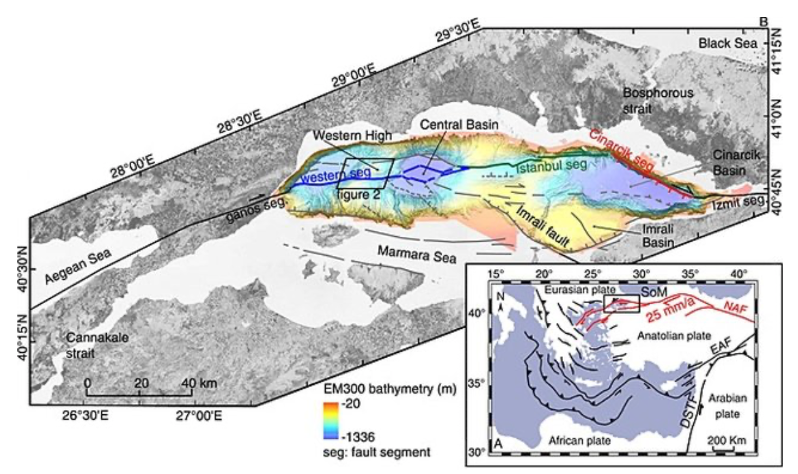
\includegraphics[width=0.5\textwidth]{images_methods/Bathy_tect.png}
    \caption{Bathymetry of the Marmara sea, taken from \cite{grall2013slip}.}
    \label{fig:bathymetry}
\end{figure}


Part of the research area consists of the Marmara sea. The topography and bathymetry are depicted in Figure \ref{fig:bathymetry} and are also considered in the simulations of this research. The maximum depth in the Marmara Sea basin lies at 1370 m below sea level. Extensive surveying of the bathymetry of the Marmara sea \cite{grall2018processed} in the context of gas migration \cite{grall2018upward}, has revealed a steep slope south of Istanbul. This slope poses an additional threat to the earthquake hazard in the region: a large event might trigger a submarine landslide, causing a tsunami (\cite{tappin2002tsunami}). Topography has been shown to have effects on the waveforms, amplitudes and timing of ground motion proxies, e.g. \cite{veeraraghavan_simulation_2020},\cite{zhang2008numerical}, \cite{pienkowska2020high}. In addition to the surface topography, the bathymetry interaction with the Marmara sea is modelled as a fluid-solid coupled domain. \cite{afanasiev2019effect} show that for higher-frequency simulations, modelling of an oceanic layer may show significant effects. 


%[!!! idea: make appears or gmrt request of the bathymetry geotif file and create a bathymetry image ??]


\section{Outlook of the research}

First we validate the model performance with respect to real events. Then we choose the Marmara region as our simulation test area, with the goal of assessing the effect of source uncertainty on ground motion proxy distribution and applying it to a region with a high seismic risk. The source is placed in the middle of the so-called Princess Island section of the fault, just below Istanbul. The following domain configurations will be considered:

\begin{itemize}
    \item 1D: 1D model with no topography
    \item 3D: 3D model with no topography
    \item 3D+topo: 3D model with topography
    \item 3D+topo+ocean: 3D model with topography and ocean solid-fluid coupling
\end{itemize}


The goal is to gradually deviate from the reference configurations in both strike, dip, rake and finally the depth of the source. Adding to this, it is investigated if the incorporation of topography and ocean implementation in the model domain are of additional influence on the spatial variabilities of the intensity measures. 

These set-ups will be analysed in a relative manner: the results show certain factors of standard deviation and amplification. This means that it can be applied and extrapolated to any event with a given magnitude. To give a short example of the implications of the results, we will shortly apply these factors to a $M_w 7.0$ hypothetical event at the given source location, and interpret the implications for the ground motions of this event on the study region. 

\end{document}